\chapter{Basic Properties of Nuclei}
\section{Rutherford Scattering Experiment}
Nucleus is discovered by Ratherford using alpha particles. Scattering experiment in which they placed a sample of alpha emitting substance behind a lead screen with a small hole in it. So that a narrow beam of alpha particle was produced. This beam was directed at a thin gold foil. A zin sulfide screen, which gives off a visible flash of light when srruck by a alpha particle was set on the side of the foil with microscope to see the flashes. It was expected that alpha particle would go right through the foil with hardly any deflection. But it was found was that although most of the alpha particle indeed were not deviated by much, a few were scattered through very large angles. Rutherford explained the result as an atom as being composed of a tiny nucleus in which its positive charge and all its mass are concentrated with the electrons some distance away with an atom being largely empty space it is easy to see why most alpha particle go right through a thin foil. How ever when an alpha particle heppens to come near a nucleus . The intence electric field there scatteres it through a large angle. The atomic electrons, being so light do not appreciably affect the alpha particles.\\

	\begin{figure}[H]
		\centering
		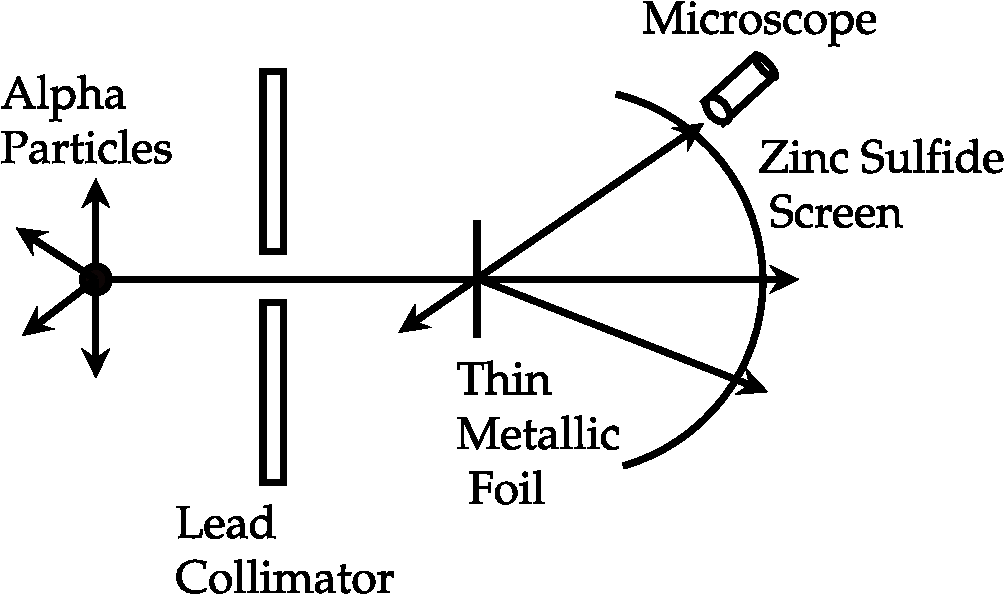
\includegraphics[height=4cm,width=7cm]{58.1-crop}
		\caption{}
		\label{}
	\end{figure}
After the discovery of protons, Rutherford proposed the nuclear model of the atom according to the model:\\
(i) The positive charge and most of the mass of the atom is concentrated in extremely small region, called the nucleus.\\
(ii) The nucleus is surrounded by electrons moving at high speeds around the nucleus in definite orbits.\\
(iii) Electrons and nucleus are held together by electrostatic force of attraction.\\\\
Later on, Rutherford supported his arguments with a mathematical model, which was based on following assumptions:\\
(1) Both the target nuclei and the $\alpha$-particles were considered as point charges.\\
(2) Nuclei is sufficiently massive to be not displaced by the encounter with the $\alpha-$ particle,\\
\subsection{Relation between scattering angle and impact parameter:}
Here the impact parameter $b$ is the minimum distance at which the $\alpha$-particle would approach the nucleus if there were no force between them. The scattering angle $\theta$ is the angle between the asymptotic incident direction of $\alpha$-particle and the asymptotic direction of the deflected $\alpha$ particle.
\begin{align*}
&\text{Impact parameter $b=\frac{Z e^2}{4 \pi \epsilon_0 k} \cot \frac{\theta}{2}$}
\intertext{Here $k=\frac{1}{2} m v^2$ is the kinetic energy of the bombarding particle. This relation shows that the scattering angle decreases as the impact parameter increases.}
&\text{In general,}\\
&\text{If $b>R \rightarrow \theta \sim 0^0$}\\
&\text{$b \sim R \rightarrow \theta$ is maximum}\\
&\text{$b<R \rightarrow \theta \sim 180^{\circ}$ back scattering}
\end{align*}
\subsection{Scattering Formula}
\begin{align*}
\text{ Angular  }&\text{scattering distribution}N(\theta)=\frac{N_l nt z^2 e^4}{(8\pi\varepsilon_0)^2r^2(KE)^2\sin^4(\frac{\theta}{2})}\\
N(\theta)&=\text{No of alpha particle per unit area that reach the screen at a scattering angle of $\theta$}\\
N_l&=\text{Total no of alpha particle that reach the screen}\\
n&=\text{No of atoms per unit volume in the foil}\\
z&=\text{Atomic numner of the foil atoms}\\
r&=\text{Distance of the screen from the foil}\\
KE&=\text{Kinetic energy of the alpha particles}\\
t&=\text{Foil thickness}
\end{align*}
\subsection{Nuclear Diamensions}
Rutherford assumed that the size of the target nucleus is small compared with the minimum distance $R$ to which incident alpha particle approch the nucleus before being deflected away. At the instant of closest approch (R), the initial $kE$ of the particle is entirely converted to electric potential energy. So that instant\\
\begin{align*}
KE_{initial}=PE&=\frac{1}{4\pi\varepsilon_0}\frac{2ze^2}{R}\\
\text{Charge of alpha particle}&=2e\\
\text{Charge of nucleus}&=ze
\end{align*}
\begin{center}
	\framebox{
		\parbox[t][1cm]{3cm}{
			
			\addvspace{-.3cm} \centering
			
			\begin{align*}
			R=\frac{2ze^2}{4\pi\varepsilon_0KE_{Initial}}
			\end{align*}} }
\end{center}
\begin{exercise}
	 Find the distance of closest approch when an alpha particle of $KE7.7 MeV$Scattered by a gold foil.
\end{exercise}
\begin{answer}
\begin{align*}
R&=\frac{2ze^2}{4\pi\varepsilon_0KE_{Initial}}\\
z(gold)&=79\\
R&=\frac{2\times79\times(16\times10^{-19})^2\times9\times10^9}{7.7\times10^6\times1.6\times10^{-19}}\\
R&=3\times10^{-14}m
\end{align*}
Radius of the gold nucleus is therefore lessthan $3\times10^{-14}$	
\end{answer}
\section{Nuclear Probes}
In order to study the nuclear size, shape and density distribution, one may employ electrons, protons and neutrons as probes.\\
The basic criterion for selecting probes is that the de Broglie wavelength of the probe should be less than or equal to the size of the object being investigated. Thus,
$$
\lambda=\frac{h}{p} \leq 2 R, \quad p \geq \frac{h}{2 R}
$$
where $R$ is the radius of the nucleus.\\
For an effective study of the nuclear density distribution, we require $\lambda \leq 2 R$\\
\textbf{Electron Beam:}\\
Electrons are the suitable probe to study the distribution of charge in a nucleus, because electrons interact with a nucleusonly through electromagnetic interaction. For this purpose high energy electron beam is required.\\
\textbf{Proton Beam:}\\
Interactions between nuclei and protons can be used to study the nuclear structure, shape and distribution of nuclear matter. Proton beams of high flux and suitable parameters are available using accelerations. However, proton-nucleus scattering results are difficult to analyze because both electromagnetic and strong interactions are present in the data.\\
\textbf{Neutron Probe:}\\
Neutrons as probe are better than protons because no coulomb interaction takes place in the scattering. But high flux and high energy neutron beams are difficult to obtain. Also, detection and measurements to protons are more difficult for neutrons as compared to protons.





\section{Nuclear Compositions}
\begin{enumerate}
\item  \textbf{Nucleons}\\All nucleus are composed of two type of particles positively charged protons and neutral neutrons jointly called as nucleons.
\item \textbf{ Atomic Number (Z)}\\
 Atomic number of an element is the no of protons in each of its atomic nuclei, which is same as the no of electrons in a neutral atom of the element.
 \item \textbf{ Mass Number (A)}\\
 Mass number of the nuclide. Total nubber of nuleons in the nucleus $A=Z+N$ $N$ is the number of neutrons in the atomic nuclens.
 \item \textbf{ Symbol of Nucleus}\\
 $^A_ZX$
 where X=chemical symbol of the element.\\
 Z=atomic number.\\
 A=mass number
 \begin{itemize}
 	\item Even-even nuclei=even proton number(Z), even neutron number $N$
 \item 	Even-odd nuclei=even protone number (Z), odd neutron number $N$
 \item 	Odd-even nuclei=odd protone number (Z), even neutron number $N$
 \item	Odd-odd nuclei=odd protone number (Z), even neutron number $N$.
 \end{itemize}
\item \textbf{Isotopes}\\
Atomic nuclei of the same element have the same number of the protons (Z) but can have different number of neutrons(N)\\
$^A_ZX$ \quad and \quad $^{A+1}_ZX$\quad  are isotopes\\\\
\textbf{Examples}\\
\textbf{1}\quad $^{13}_6C$\quad and \quad $^{14}_6 C$\\\\
\textbf{2)}\quad $^1_1H,\quad^2_1H,\quad^3_1H$\\
 Hydrogen deuterium and titrium are the isotops of Hydrogen\\
\begin{figure}[H]
	\centering
	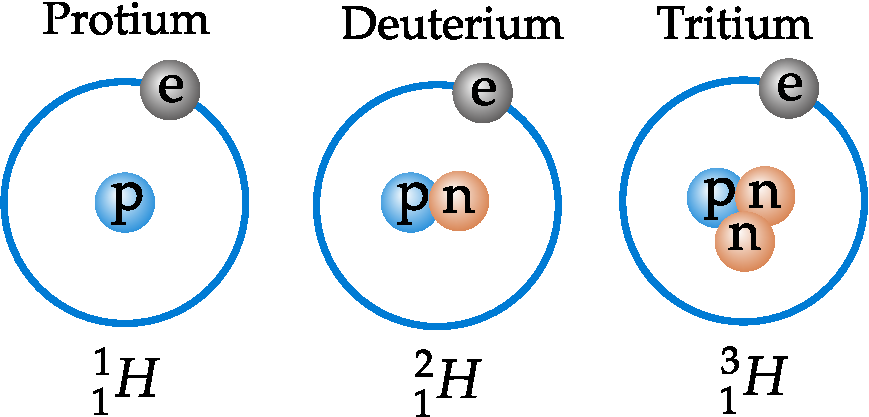
\includegraphics[height=2.8cm,width=6cm]{20.11-crop}
	\caption{}
	\label{}
\end{figure}
\begin{note}
	\textbf{1)}\quad $^1_2 H$ -\quad deuterium is stable, and is called heavy water\\\\
		\textbf{2)}\quad $^3_1H$-Tritium is radio active, which are found in atmosphere by the nuclear reactions of cosmic rays in the atmosphere.  Only about $2kg$ of tritium is present at any time of earth.
\end{note}
\item  \textbf{Isobars}\\
Atomic nuclei with equal mass number $A$,but different proton number $Z$ .
\begin{itemize}
	\item $^A_Z X$ \  and\ $^A_{Z+1} Y$ are Isobars.
\end{itemize}
\textbf{example}\quad $^{14}C$\  and\  $^{14} N$
\item  \textbf{Isotones}\\
Atomic nuclei with equal neutron numbers but different atomic number $Z$.
\begin{itemize}
	\item $^A_Z X$ \  and\ $^{A+1}_{Z+1} Y$ are Isotons.
\end{itemize}
\item  \textbf{Atomic Masses}\\
Atomic masses refer to the masses of neutral atoms, not of bare nuclei. Thus an atomic mass always include the mass of $Z$ electrons. Atomic mass are expressed in mass units (u). Which is equal to $\frac{1}{12}$ of the mass of neutral atom of \ $^{12}_6 C$\\
$$n=\frac{1}{12} m\left({ }{^{12}_6C}\right)=\frac{1 \mathrm{~g}}{N_{A}}=1.660 \times 10^{-27} \mathrm{~kg} .$$
\begin{center}
	\framebox{
		\parbox[t][0.5cm]{3.5cm}{
			
			\addvspace{-0.5cm} \centering
			
			\begin{align*}
			1 n=1.660 \times 10^{-27} kg
			\end{align*}} }
\end{center}
Where $N_A$ is the avagadro number, equal to $6.023 \times 10^{23}$. Then the mass of $^{12}_6C$ atomic is excatly $12 u$. The energy equalent of mass unit is $931.49 \mathrm{MeV} .$\\\\
\renewcommand*{\arraystretch}{1.5}
\begin{tabular}{c|c|c|c|}
	\hline
	Particle & Mass(Kg) & Mass(u) & Mass($Me V/C^2$)\\
	\hline
	Proton & $1.6726 \times 10^{-27}$ & $1.007276$ & $938 \cdot 28$\\
	\hline
	Neutron & $1.6750 \times10^{-27}$ & $1.008665$ & $939.57 .$\\
	\hline
	Electron & $9.1095 \times 10^{-31}$ & $5.486 \times 10^{-4}$ & $0.511$\\
	\hline
	$^1_1 H$ atom & $1.6736 \times 10^{-27}$ & $1.007825$ & $938.79$\\
	\hline
\end{tabular}\\\\\\
$\Rightarrow$ \textbf{How to convert mass in $Kg$ in to mass in $u$ and $MeV/C^2$}\\
Take the example as proton with mass $1.6726 \times 10^{-27}$ 
\begin{align*}
\text{Mass in u}&=\frac{1.6726 \times 10^{-27}}{1u}\\
&=\frac{1.6726 \times 10^{-27}}{1.660 \times 10^{-27}}=1.007276u\\
\text{Mass in}\  \frac{\mathrm{MeV}}{C^2} &=1.007276 \times 931.49 \mathrm{MeV}\\
&=938.28 \mathrm{MeV} / \mathrm{c}^{2} 
\end{align*}
\end{enumerate}
\section{Nuclear Properties}
\begin{enumerate}
	\item \textbf{Nuclear charge distribution}\\
 The central nuclear charge density is nearls the same for all nuclei. Nucleons do not seem to congregate near the center of the nucleus. but instead have a fairly constant distribution out to the suriace. Thus the number of nucleons per unit volume is roughly constant:\\
\begin{figure}[H]
	\centering
	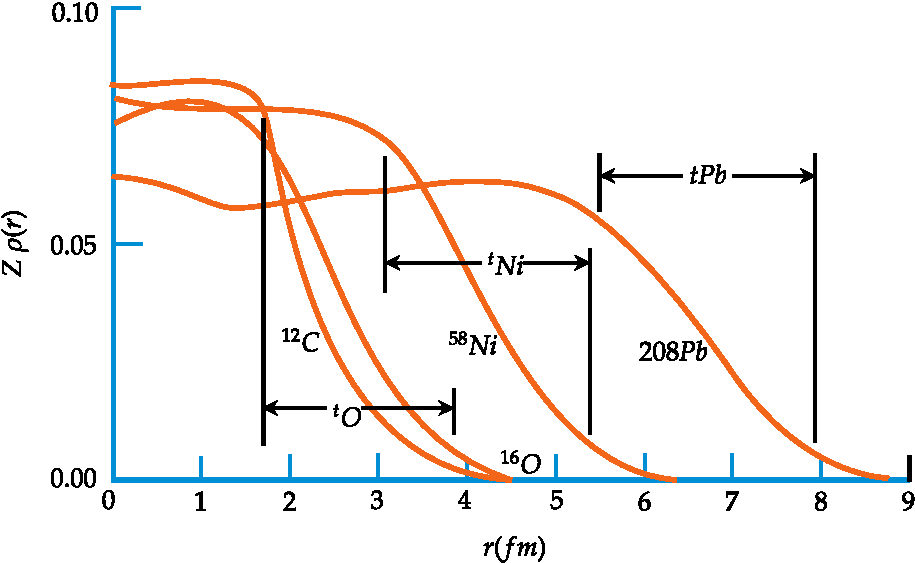
\includegraphics[height=5.4cm,width=10cm]{diagram-20220307(4)-crop}
	\caption{ The radial charge distribution of several nuciei determined from electron scattering. The skin thickness $t$ is shown for $O, N i$, and $P b$; its value is roughly constant at $2.3 \mathrm{fm}$. The central density changes very littie from the lightest nuclei to the heaviest.}
	\label{ref.nuclear}
\end{figure}
 Figure $\ref{ref.nuclear}$ also shows how diffuse the nuclear surface appears to be. The charge density is roughly constant out to a certain point and then drops relatively slowly to zero. The distance over which this drop occurs is nearly independent of the size of the nucleus, and is usually taken to be constant. We define the skin thickness parameter $t$ as the distance over which the charge density falls from $90 \%$ of its central value to $10 \%$. The value of $t$ is approximately $2.3 \mathrm{fm}$.
	\item \textbf{Size of the Nucleus}\\
It is possible to obtain the size of the nucleus through Ruther ford experiment. We can calculate the size of a nucleus by obtaining the point of closest approach of alpha particle. The size of the nucleus is smaller than $10^{-14}m$. Formula to measure the size of the nucleus can be determined. The volume of the nuclens is proportional to  $A$ \\
\begin{align*}
\frac{4}{3}\pi R^3&\propto A\quad\text{($R$ is the radius) }\\
R&=R_0 A^\frac{1}{3}\\
\text{ Where }R_0&= 1.2\times 10^{-15}m=1.2 fm
\end{align*}
\text{$fm$\ is femtometer (fm)and sometimes called fermi}\\
\textbf{Examples}
\begin{enumerate}
	\item $ \text{Radius of}\ ^{12}_6 C\  \text{nucleus}$
$R\approx(1.2)(12)^\frac{1}{3}fm=2.7fm$
\item $ \text{Radius of }^{107}_{47}Ag$
$R\approx(1.2)(107)^\frac{1}{3}=5.7fm$
 \item $ \text{Radius of }^{238}_{92}u$
$R\approx(1.2)(238)^\frac{1}{3}=7.4fm$
\end{enumerate}
\item \textbf{Density}\\
Density of $^{12}_6C$ nucleus can be find out as
\begin{align*}
\text{Density } \rho &=\frac{mass}{\text { volume. }}\\
\text{Mass of $C$ nuclei is }&=12 u\text{(neglect the masses and binding energies of six electrons)}\\
\rho&=\frac{12\times1.66\times10^{-27}Kg}{\left(\frac{4}{3}\pi \right)\left(2.7\times 10^{-15} m \right)^3  }\\
&=2.4 \times 10^{17} Kg l \mathrm{~m}^{3}
\end{align*}
Which is equalent to 4 billion tones per cubic inch. So it is approximately taken the same for all nuclei.
\begin{center}
	\framebox{
		\parbox[t][0.5cm]{3.5cm}{
			
			\addvspace{-0.5cm} \centering
			
			\begin{align*}
			\text{Density}S=2.4\times10^{17}Kg/m^3
			\end{align*}} }
\end{center}
for all nuclei
\item \textbf{Spin of Nucleus}\\
Proton and neutrons like electrons are fermions with spin quantum number of $S=\frac{1}{2}$
\begin{enumerate}
	\item \textbf{Spin Angular Momenta S(individual)}$\left. \right. $\\
\begin{minipage}{0.45\textwidth}
	\begin{align*}
	S_{p/n}&=\sqrt{S(S+1)}=\sqrt{\frac{1}{2}\left(\frac{1}{2} +1\right) \hbar}\\
	S_{p/n}&=\frac{\sqrt{3}}{2}\hbar\\
	\text{and}\quad
	S_z&=m_s\hbar=\pm\frac{1}{2}\hbar
	\end{align*}
\end{minipage}
\begin{minipage}{0.30\textwidth}
	\begin{figure}[H]
		\centering
		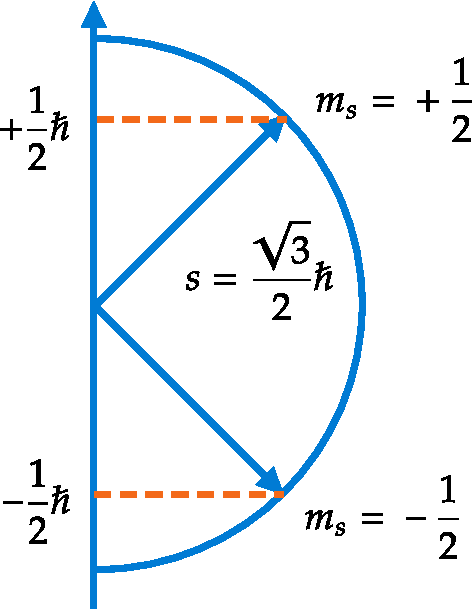
\includegraphics[height=4cm,width=3.5cm]{NC 03-crop}
		\caption{}
		\label{Decreasing Function}
	\end{figure}
\end{minipage}\\
$m_s$ is the spin magnetic quantum number $m_s=\pm\frac{1}{2}$. $S_z$ is $z $ component of spin angular momentum.
 \textbf{Total Spin angular moment of Nucleus}\\
 \begin{enumerate}
 	\item Spin of Hydrogen $=\frac{1}{2}$\\
 	\item Nuclei with both $P$and $n$ are even ($A,Z$ even) have total 
 	Spin $=0$\\
 	\textbf{Eg:}\quad $^2_2 H,\  ^{12}_6 C,\ ^{16}_8 O$\\
 	\item Nuclei with Both $P$ and $n$\ are odd ($Z$\ odd,\ $A$ even) have 
 	integral spin\\
 	\textbf{Eg:}\quad $^2_1 H,\  ^{14}_7 N,\ ^{10}_5 B$\\
 	\item nuclei With an odd A(mass number) have half integral spin\\
 	\textbf{Eg:}\quad $^1_1 H,\quad ^{15}_7 N$\ (spin$=\frac{1}{2}$),\quad$^{17}_8 O$(spin$=\frac{5}{2}$)\\
 \end{enumerate}
\begin{align*}
\text{Total spin }&\text{of a nucleus can be represented by letter $I$}\\
\therefore \quad I&=\sqrt{I(I+1)}\hbar\\
\text{$I$ may be }&\text{zero integral or half integral.}\\
\text{For $I=1$, }&\text{the possible $I_2$ values are $-1,0,+1$ and can be represented as }
\end{align*}
\begin{figure}[H]
	\centering
	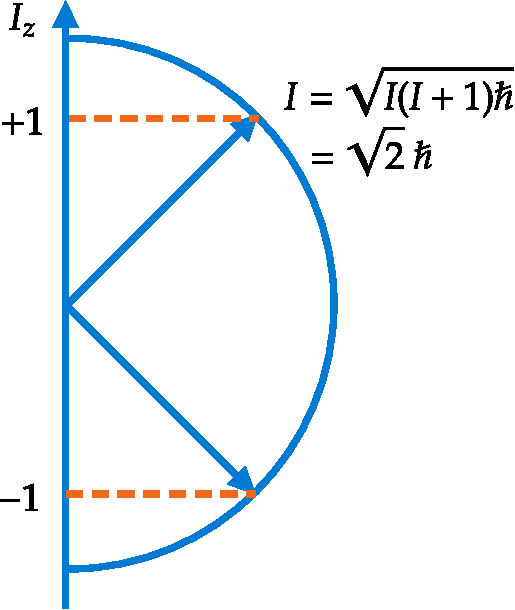
\includegraphics[height=4cm,width=3.5cm]{NC 04-crop}
	\caption{}
	\label{}
\end{figure}
	\item \textbf{Spin Magnetic Momenta(individual)}\\
	 The individual spin magnetic momenta of proton and neutron can be represented as,\\
	\begin{align*}
	\mu_{P_{2}}&=\pm 2.793 \mathrm{N}\\
	\mu_{N_{2}}&=\mp 1..913 \mathrm{N}
	\end{align*}
	The spin magnetic moment $\mu_P$ of the proton is in the same direction as its spin angular momentum. $N$ and in the case of neutron $\mu_{N}$ opposite to $S$.\\\\
	\begin{figure}[H]
		\centering
		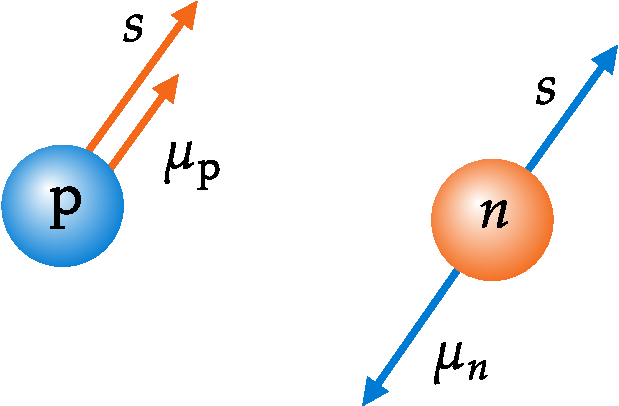
\includegraphics[height=2.5cm,width=4cm]{CN 05-crop}
		\caption{}
		\label{}
	\end{figure}
\textbf{Total spin magnetic moment of the nucleus}\\
A charged particle spinning about ab axis constitutes a circular electric current which in turn produces a magnetic dipole .In other words the spinning particle behaves as a tiny bar magnet placed along the spin axis.The strength of the magnet for a point charge can be shown to be 
\begin{align*}
\mu&=\frac{q}{2m}I=\frac{q\sqrt{I(I+1)}}{2m}\frac{h}{2\pi}=\frac{qh}{4\pi m}\sqrt{I(I+1)}Am^2
\intertext{We can remove the fiction that nuclei are point charges the above equation become modified by the inclusion of a numerical factor G.}
\mu&=\frac{Gqh}{4 \pi m}\sqrt{I(I+1)}JT^{-1}\\
\text{Nuclear G factors }&\text{cannot be calculated in advance and are obtained only experimentally.}
\intertext{Nuclear dipoles are conveniently expressed in terms of nuclear magneton $\beta_N$ which is defined in terms of mass and the charge of the proton.}
\beta_N&=\frac{eh}{4m_p \pi}=5.050 \times 10^{-2 7} \mathrm{~J}{T}^{-1}=3.152 \times 10^{-8} \mathrm{eV} T^{-1}\\
\text{Thus for a nucleus of mass}&\text{ pe( M and charge where p is the number of proton)we would write}\\
\mu&=\frac{Gpe}{2M}\sqrt{I(I+1)}\frac{h}{2 \pi}=\frac{Gm_pp}{M}\beta_N\sqrt{I(I+1)}\\
&=g\beta_N\sqrt{I(I+1)}
\end{align*}

where we have collected the parameters $\frac{Gm_pp}{M}$ in which $m_p$ is the protonic mass into a factor g which is the characterstics of each nucleus.This factor has value up to about six and is positive for nearlly all known nuclei.\\
The dipole will plainly have components along a reference direction goverened by the $I_z$ values\\
$$\mu_{z}=g\beta_NI_z$$
\end{enumerate}
\begin{note}	
 \textbf{1)}\quad A nucleon in a more complex nucleus may have orbital angular momentum  due to motion inside the nucleus as well as the spin angular momentum. The total angular momenta of such a nucleus is the vector sum of the spin and orbital angular momenta of its nucleus as in the analogous case of the electrons of the atom.\\\\
 	\textbf{2)}\quad \textbf{Larmor Frequency}\\
 	When a nucleus whose magnetic moment has the $Z$ component $\mu_{Z}$ is in a constant magnetic field $B$. The magnetic $PE$ of the nucleus ,\\
 	$$u_{m}=-\mu_{2} B$$
 	Therefore in a magnetic field the angular momentum state of the nucleus is split in to components according to the $m_s$values . Now consider the splitting of angular momenta of the nucleus due to a single proton.\\
 	\begin{figure}[H]
 		\centering
 		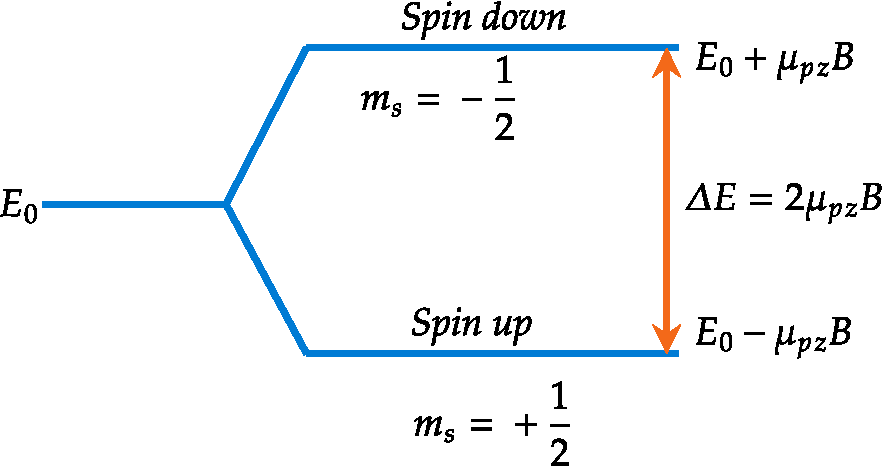
\includegraphics[height=3.5cm,width=7.5cm]{CN 06-crop}
 		\caption{}
 		\label{}
 	\end{figure}
 	\begin{align*}
 	B&=0\hspace{1cm} B>0\\
 	\Delta E&=2 \mu_{p_{Z}} B
  \intertext{	A Proton with this energy will be emitted when a proton in the upper state flips its spin to fall to the lower state. A proton in the lower state can be raised to the upper one by absorbing a photon of the energy. The photon frequency $\nu_L$ that corresponds to $\Delta E$is,}
 \nu_{L}&=\frac{\Delta E}{h}=\frac{2 \mu P_{Z} B}{h}\\
 \text{This frequency}&\text{ is called Larmor frequency}
 		\end{align*}
 	
\end{note}
\begin{exercise}
	 (a)\quad Find the energy difference between the spin up and spin down states of a proton in a magnetic field of $B=1\cdot T$ \\
	(b)\quad What is the Larmor frequency?
\end{exercise}
\begin{answer}
	\begin{align*}
	(a)\quad
	\delta E&=2\mu_{P_{Z}}B=2\times(2.793)\times \left(3.153\times10^-8\frac{eV}{T} \right) \times1T\\
	&=1.761\times10^-7 eV\\
	(b)\quad \nu_{L}&=\frac{\Delta e}{h}=\frac{1.761\times10^{-7}}{4.136\times10^{-15}eV\cdot S}\\
	&=4.258\times10^7Hz=42.58MHz
	\end{align*}
	Which is in the lower end of the microwave part of the spectrum.
\end{answer}
\item \textbf{Electric Moment of Nuclei}
We have seen that the atomic nucleus is a positively charged body of finite dimentions. We know that any distribution of electric charge produce an electric potential $\phi(r,\theta)$at a distance at $r$ in the $Z$ direction. This potential $\phi(r,\theta)$ due to an azimuthally symmetric distribution of electric charges can be expanded in ascending powers of $\frac{1}{r}$
$$\phi(r,\theta)=\frac{1}{r}\sum_{n=o}^{\infty}\frac{a_n}{r^n}P_n(\cos\theta)$$
$P_n$ are the legendre polynomial\\
$I^{st}$ term in the expansion curresponds to potential due to electric monopole. Which is a point charge $+Ze$. The second term corresponds to potential due to electric dipole. But the electric dipole moment of a nucleus is zero for ground state and nondegenerate excited state of the nucleus. Similarly the electric moment of all odd orders (Eg: Octapolemoment)are zeros for the nucleus. The third term in the expansion is called quadrapole moment.
\item \textbf{Electric Quadrapole Moment}\\
Atomic nuclei with spin $=0$ have zero quadrapole moment and sphererical in shape. \\
Atomic nuclei with spin $>1$ have quadrapole moment other than zero. It shows that their form is not strictly spherical. The quadrapole moment has a plus sign if the nucleus is  extended along  the spin axis (a spindle shape body) and minus sign if the nucleus is extented in a plane $\perp$ to the spin axis (a lenticular body). A nucleus posessing a quadrapole moment produces nonspherically symmetrical field. Let $\theta_0$ be the intricsic quadrapole moment of a nucleus. Then 
\begin{align*}
Q_0&=\frac{1}{e}\int(3{Z^\prime}^2-{r^\prime}^2)\rho(r^\prime)d\tau^\prime
\intertext{Where integration is carried out over the entire volume of the nucleus. $r^\prime(x^\prime,y^\prime,z^\prime)$ is the distance measured from the center of mass of the nucleus.}
\text{For a spherically}&\text{ symmetric charge distribution.}\\
\rho(r^\prime){x^\prime}^2d\tau^\prime&=\int \rho(r^\prime){y^\prime}^2d\tau^\prime=\int \rho(r^\prime){z^\prime}^2d\tau^\prime=\frac{1}{3}\int \rho(r^\prime){r^\prime}^2d\tau^\prime\\
\text{Therefore $\theta_0$}&=\text{$0$for spherical nucleus.}\\
\text{For a nonsperical }&\text{nucleus $\theta$ and $\theta_0$ is related as,}\\
Q&=Q_0\left( \frac{I(2I-1)}{(I+1)(2I+3)}\right) \\
\text{Where $I$ is the total }&\text{angular momentum (spin)}\\
\text{If}\quad Q_0>0, &\int \rho(r^\prime){z^\prime}^2d\tau^\prime>\frac{1}{3}\int \rho(r^\prime){r^\prime}^2d\tau^\prime\\
\text{Such nucleus is eleongated }&\text{ along the $z^\prime$ axis (cigar shaped) is called prolate spheroid.}\\
\text{If}\quad Q_0<0, &\int \rho(r^\prime){z^\prime}^2d\tau^\prime<\frac{1}{3}\int \rho(r^\prime){r^\prime}^2d\tau^\prime\\
\text{Such nucleus is called }&\text{oblate spheroid (pancake shape)}
\end{align*}
\begin{figure}[H]
	\centering
	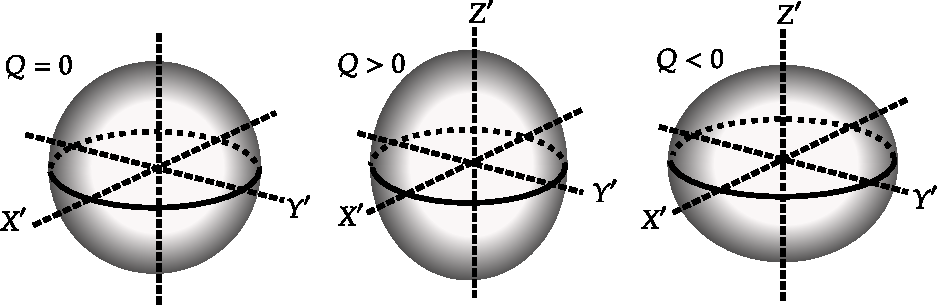
\includegraphics[height=4cm,width=10cm]{diagram-20220307(5)-crop}
	\caption{}
	\label{}
\end{figure}
\item \textbf{Isospin}
\begin{align*}
\text{For a given }&\text{nucleus, the value of $T_3$ or $T_Z$ is just the minus one half of the neutron excess}\\
T_Z&=-\frac{1}{2}(N-Z)=-\frac{1}{2}(A-2 Z)\\
\text{In a set of }&\text{isobars of a given $A$, a member $X$ will have an isospin $T_{Z, \text { max }}$ largest among the set. For this}\\
T_{Z, \text { max }}&=T=\frac{1}{2}\left(Z_X-N_X\right)\\
\text{This $T$ }&\text{is corresponding to $(2 T+1)$ states.}\\
\text{These states }&\text{are  corresponding to different values of $T_Z$ and hence have different charges}\\
Z&=\frac{A}{2}+T_Z
\end{align*}
\textbf{Example:} Set of isobars ${ }^{14} C,{ }^{14} N,{ }^{14} O$ are representing three states corresponding to $T=1$ and have $T_z=-1,0,+1$
\begin{align*}
&{ }_6^{14} C\hspace{4cm}{ }_7^{14} \mathrm{~N}\hspace{4cm}{ }_8^{14} O\\
&T_z=-\frac{1}{2}(14-12)=-1 \hspace{1cm} T_z=-\frac{1}{2}(14-14)=0 \hspace{1cm} T_z=-\frac{1}{2}(14-16)=+1\\
&T_{Z, \max }=+1=T\\
&\text{Total states }=(2 T+1)=3
\end{align*}
\textbf{Example:}
\begin{align*}
&\qquad{ }_1 H^3 \hspace{6cm} { }_2 \mathrm{He}^3\\
&T_3=-\frac{1}{2}(3-2)=-\frac{1}{2} \hspace{2cm}T_3=-\frac{1}{2}(3-4)=+\frac{1}{2}\\
&T_{3, \max }=+\frac{1}{2}=T \qquad \text { Total states }=(2 T+1)=2\\
&\text { Note: Members of the same isospin multiplet have the same spin-parity. }
\end{align*}
\end{enumerate}
\section{Stable Nuclei}
\begin{figure}[H]
	\centering
	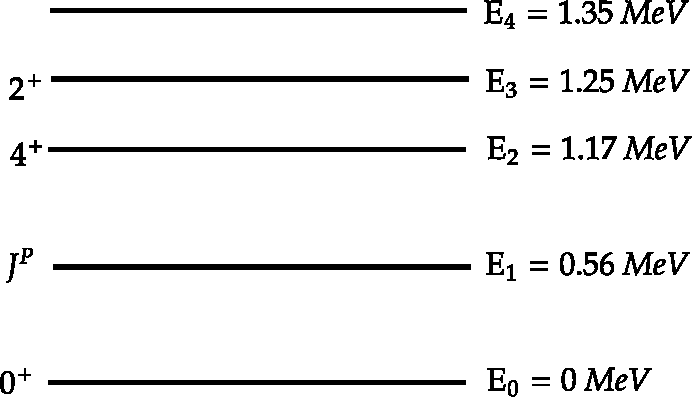
\includegraphics[height=4.2cm,width=4cm]{NP-1}
	\caption{Neutron-proton diagram for stable nuclides}
	\label{}
\end{figure}
Not all combination of neutrons and protons form stable nuclei. In general, light nuclei $(A<20)$ contain equal numbers of neutrons and protons, while in heavier nuclei the proportion of neutrons becomes progressively greater. This is evident in figure as shown below, which is plot of $N$ versus $Z$ for stable nuclides.\\
The tendency for $N$ to equal $Z$ follows from the existence of nuclear energy levels. Nucleons, which have spin $1 / 2$, obey\\
exclusion principle. As a result, each energy level can contain two neutrons of opposite spins and two protons of opposite spins. Energy levels in nuclei are filled in sequence, just as energy levels in atoms are, to achieve configurations of minimum energy and therefore maximum stability. Thus the boron isotope ${ }_5^{12} \mathrm{~B}$ has more energy than the carbon isotope ${ }_6^{12} \mathrm{C}$ because one of its neutrons is in a higher energy level, and ${ }_5^{12} \mathrm{~B}$ is accordingly unstable. If created in a nuclear reaction, a ${ }_5^{12} \mathrm{~B}$ nucleus changes by beta decay into a stable ${ }_6^{12} \mathrm{C}$ nucleus in a fraction of second.
\begin{figure}[H]
	\centering
	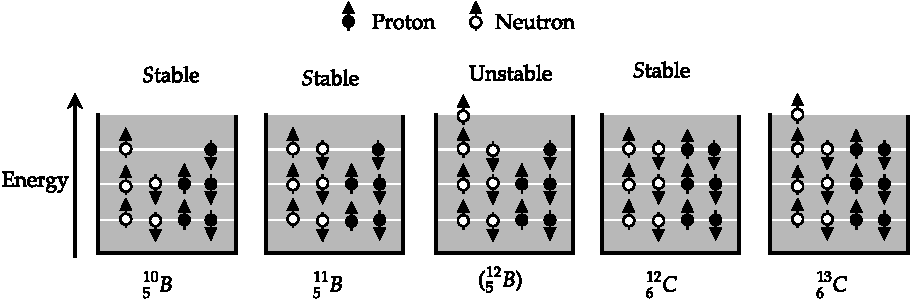
\includegraphics[height=4.5cm,width=14cm]{NP-2}
	\caption{Simplified energy level diagrams of some boron and carbon isotopes.}
	\label{}
\end{figure}
The preceding argument is only part of the story. Protons are positively charged and repel one another electrically. This repulsion becomes so great in nuclei with more than 10 protons or so that an excess of neutrons, which produce only attractive forces is required for stability. Thus the curve departs more and more from $N=Z$ line as $Z$ increases.\\
Sixty percent of stable nuclides have both even $Z$ and even $N$; these are called "even-even" nuclides. Nearly all the others have either even $Z$ and odd $N$ ("even-odd" nuclides) or odd $Z$ and even $N$ ("odd-even" nuclides) with the numbers of both kinds being about equal. Only five stable odd-odd nuclides are known: ${ }_1^2 \mathrm{H},{ }_3^6 \mathrm{Li},{ }_5^{10} \mathrm{~B},{ }_7^{14} \mathrm{~N}$ and ${ }_{73}^{180} \mathrm{Ta}$. Nuclear abundances follow a similar pattern of favoring even numbers for $Z$ and $N$.\\
These observations are consistent with the presence of nuclear energy levels that can each contain two particles of opposite spin. Nuclei with filled levels have less tendency to pick up other nucleons than those with partially filled levels and hence were less likely to participate in the nuclear reactions involved in the formation of elements.\\
Nuclear forces are limited in range, and as a result nucleons interact strongly only with their nearest neighbors. This effect is referred to as the \textbf{saturation} of nuclear forces. Because the coulomb repulsion of protons is appreciable throughout the entire nucleus, there is a limit to the ability of neutrons to prevent the disruption of large nucleus. This limit is represented by the bismuth isotope ${ }_{83}^{209} \mathrm{Bi}$, which is the \textbf{heaviest stable} nuclide.\\
All nuclei with $Z>83$ and $A>209$ spontaneously transform themselves lighter ones through the emission of one or more alpha particles, which are ${ }_2^4 \mathrm{He}$ nuclei:\\
\textbf{Alpha Decay }
$${ }_{\mathrm{Z}}^{\mathrm{A}} \mathrm{X} \rightarrow{ }_{\mathrm{Z}-2}^{\mathrm{A}-4} \mathrm{Y}+{ }_2^4 \mathrm{He}$$
Since an alpha particle consists of two protons and two neutrons, an alpha decay reduces the $Z$ and $N$ of the original nucleus by two each. If the resulting daughter nucleus has either too small or too large a neutron/proton ratio for stability, it may beta-decay to a more appropriate configuration.\\
In negative beta decay, a neutron is transformed into a proton and an electron is emitted:\\
\textbf{Negative Beta Decay}
$$
n^0 \rightarrow p^{+}+e^{-}
$$
In positive beta decay, a proton becomes a neutron and a positron is emitted:\\
\textbf{Positron emission}
$$
p^{+} \rightarrow n^0+e^{+}
$$
Thus negative beta decay decreases the proportion of neutrons and positive beta decay increases it. A process that competes with positron emission is the capture by a nucleus of an electron from its innermost shell. The electron is absorbed by a nuclear proton which is thereby transformed into neutron:\\
\textbf{Electron Capture}
$$
p^{+}+e^{-} \rightarrow n^0
$$
Figure below shows how alpha and beta decays enable stability to be achieved.
\begin{figure}[H]
	\centering
	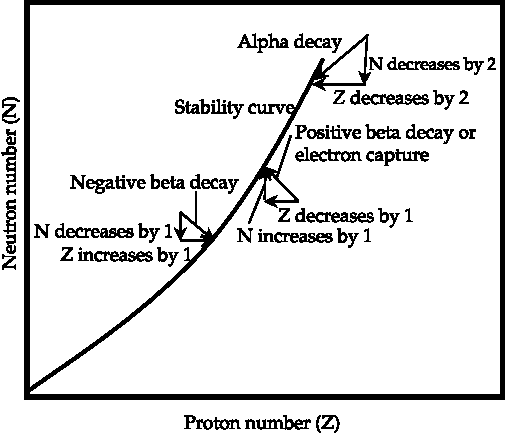
\includegraphics[height=7cm,width=7.5cm]{NP-3}
	\caption{Alpha and beta decays permit an unstable nucleus to reach a stable configuration.}
	\label{}
\end{figure}
\section{Statistics}
When we group together several particles to make a large quantum system, like several nucleons inside nuclei, a new quantum effect arises if the particles are indistinguishable from one another. Consider a system of two indistinguishable nucleus say 1 and 2. Suppose ' 1 ' nucleon is described by coordinate $r_1$ and is in the state $\psi_1\left(\vec{r}_1\right)$ and '2' nucleon is described by coordinate $r_2$ and is in the state $\psi_2\left(\vec{r}_2\right)$. The combined wave function of two nucleon system is as follows:
$$
\psi(1,2)=\psi_1\left(\vec{r}_1\right) \psi_2\left(\vec{r}_2\right)
$$
If the particles are interchanged, then new wave function is:
$$
\psi(2,1)=\psi_2\left(\vec{r}_2\right) \psi_1\left(\vec{r}_1\right)
$$
In both cases, the probability density $|\psi(1,2)|^2$ and $|\psi(2,1)|^2$ will be same, because there is no way to distinguish between '1' and ' 2 ' nucleon.

The exchanged wave function $\psi(2,1)$ can at most differ only in sign from original wave function
$$
\begin{aligned}
&\psi(1,2)=+\psi(2,1) \\
&\psi(1,2)=-\psi(2,1)
\end{aligned}
$$
If the exchange does not change sign, the wave function is symmetric. If the exchange changes the sign, the wave function is anti-symmetric.

All particles in the first category are called Bosons and those in the second category are called fermions. Without any exception, bosons are integral spin $(0,1,2, \ldots)$ and fermions are half integral spin $\left(\frac{1}{2}, \frac{3}{2}, \frac{5}{2}, \ldots\right)$ particles.\\
	\begin{table}[H]
	\centering
	\renewcommand*{\arraystretch}{1.5}
	\begin{tabular}{|p{7cm} |p{7cm}|}
\hline	\textbf{Bosons}&\textbf{Fermions}\\\hline
	1.Bosons follow BE-statics&1. Fermions follow F-D statistics\\\hline
	\text { 2. They have integral spins }(0,1,2, \ldots)&\text { 2. They have half integral spin }$\left(\frac{1}{2}, \frac{3}{2}, \frac{5}{2}, \ldots\right)$\\\hline
	3. They do not follow Pauli's Exclusion principle&3. They do not follow Pauli's Exclusion principle\\\hline
	4. Wave function is symmetric $\psi(1,2)=+\psi(2,1)$&4. Wave function is antisymmetric $\psi(1,2)=-\psi(2,1)$\\\hline
	Examples: pi-mesons, $K$-mesons, photons and all nuclei having even mass number ${ }_1 D^2,{ }_2 H e^4,{ }_8 O^{16},{ }_{16} S^{32}$&Example: $e^{-}, e^{+}, p, n, \mu$-mesons and nuclei of odd mass number
	$$
	{ }_1 H^1,{ }_3 L i^7,{ }_9 F^{19},{ }_{11} N a^{23},{ }_{17} C l^{35}
	$$\\\hline
	\end{tabular}
\end{table}
\section{Parity}
Parity relates to the symmetry of the wave function that represents the system. If the wave function is unchanged, when the coordinates $(x, y, z)$ are replaced by $(-x,-y,-z)$ then the system has a parity of $+1$. If the wave function has its sign changed, when the coordinates are reversed, then the system has parity of $-1$.\\
If we write
$$
\psi(x, y, z)=P \psi(-x,-y,-z)
$$
we can regard $P$ as a quantum number characterizing $\psi$ whose possible values are $+1$ and $-1$.\\
It has been observed that spatial part of $\psi$ of a particle does not change its sign on reflection if the angular momentum quantum number " $l$ " is even.\\
As a general rule \textbf{Parity} $=(-1)^l$\\
For a system of particles Parity is even if $\sum l$ even and Parity is odd if $\sum l$ odd.
\section{Binding Energy}
Binding energy $BE$, the energy released when free nucleons are bound together to form a nucleus. SI unit is the Joule(J). Usually the binding energy is given in MeV. The mass of a stable atomic nucleus is smaller than the sum of the masses of the constituent nucleons. The missing mass is converted in to its energy equivalent called binding energy. The greater its $BE$ the more the energy that must be supplied to breake up the nucleus. The binding energy $E_b$in MeV  of the nucleus $^A_ZX$ is given by.
\begin{align*}
E_b&=\left[ zm(^1_1H)+NM(n)-m(^A_ZX)\right]\left(931.49\  MeV/u \right)  \\
\text{Where}\\
m(^1_1H)&=\text{Is the atomic mass of }^1_1H\\
&=1.007825 u\\
Z&= \text{ Atomic number}\\
N&= \text{No of neutrons}\\
M(n)&=\text{Mass of neutron}\\
&=1.008665 u\\
^A_ZX&= \text{Atomic mass of element }X
\end{align*}
\section{Binding Energy Per Nucleon}
The binding energy per nucleon for a given nucleus is an average found by dividing its total binding energy by the no of nucleons it contain. The range for the stable nuclei is from $2.224\ MeV$ for $^2_1H$\ (deuterium)\ to $1640\ MeV$ for $^{209}_{83}B_1$. The binding energy per nucleon for $^2_1H$\ is $\frac{2.2}{2}=1.1MeV/\text{nucleon}$ and for $^{209}_{83}B_1$\ is $\frac{1640}{209}=7.8 MeV/\text{nucleon}$.\\
The graph binding energy per nucleon against number of nucleons (A) is called binding energy curve.
\begin{exercise}
	The binding energy of neon isotope $^2_{10}Ne$\ is $160.647\ MeV$. Find its atomic mass.
\end{exercise}
\begin{answer}
	\begin{align*}
	\text{Here}\quad Z=10\quad N&=10,E_b=160.647 \ MeV\\
	\left[ Zm(^1_1H)+Nm(n)\right] &-\frac{E_b}{931.49}\\
	=19.992 \ u
	\end{align*}
\end{answer}
\subsection{Binding Energy Curve}
\subsubsection{Conclusions Drawn From the Curve}
\begin{figure}[H]
	\centering
	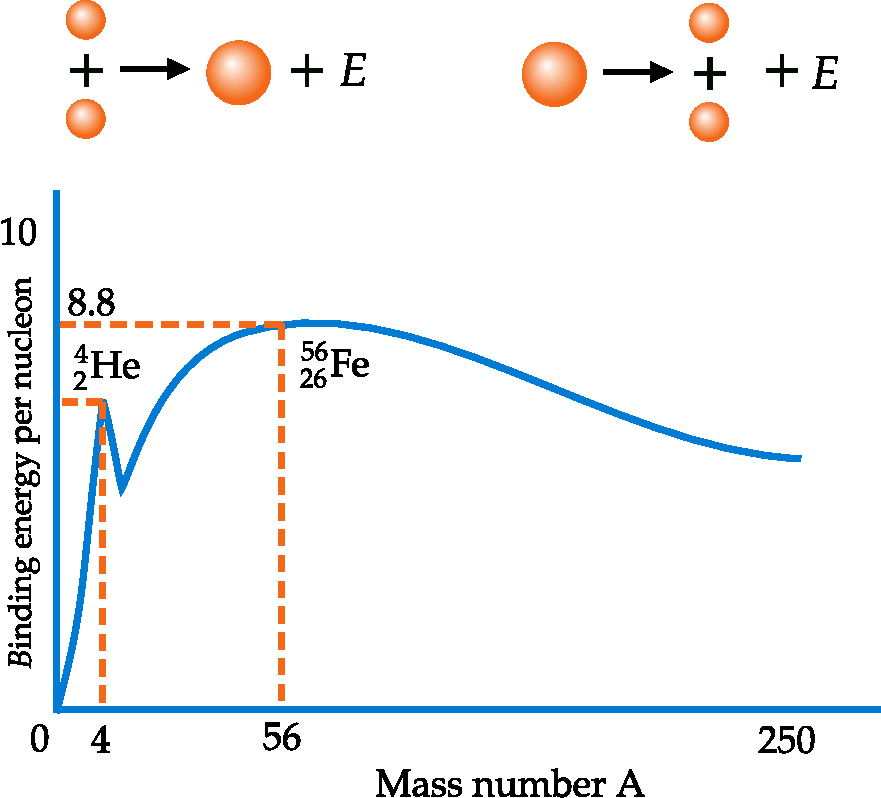
\includegraphics[height=7cm,width=7.5cm]{NC 07-crop}
	\caption{}
	\label{}
\end{figure}
\textbf{1)} \quad Binding energy per nucleons is almost constant except for very small $A$\\
The peak at $A=4$ corresponds to the exceptionally stable $^4_2He$ nucleus. Which is the alpha particle \\\\
\textbf{2)}\quad The graph has its maximum of $8.8\ MeV/\text{nucleon}$. When the total number of neucleon is $56$. That is $^{56}_{26}Fe$\ is $160.647\ MeV$ an iron isotope.\\\\
\textbf{3)}Suppose if we split a heavy nucleus (At the last part of the graph) in to two medium sized ones, each of the nuclei will have more binding energy per nucleon than the original nucleus have. A lot extra energy will be given off.\\
\textbf{Eg:}\quad If uranium nucleus $^{235}_{92}U$\ is broken into smaller nuclei. The binding energy difference per nucleon is $0.8\ MeV$\\
Then total energy given off $=0.8\times235=188\ MeV$. A single nucleus can given this much of energy. Which is very large.\\
Such splitting of heavy nucleus in to smaller one with large amount of energy is called nuclear fission.\\\\
\textbf{4)}\quad Suppose that we are joining two light nuclei together to give a single nucleus of medium sized one will also given off large amount of energy.\\
\textbf{Eg:} \quad If two $^2_1H$( deuterium )nuclei combine to form a  $^4_2He$\ Helium nucleus about $23MeV$\ energy is released. Such process is called Nuclear Fission. Is the main energy source of the sun and other stars.

\newpage
\begin{abox}
	Practise set-1
\end{abox}
\begin{enumerate}
	\item  The radius of a ${ }_{29}^{64} \mathrm{Cu}$ nucleus is measured to be $4.8 \times 10^{-13} \mathrm{~cm}$. The radius of a ${ }_{12}^{27} \mathrm{Mg}$ nucleus can be estimated to be
	 \begin{tasks}(2)
		\task[\textbf{a.}]$2.86 \times 10^{-13} \mathrm{~cm}$
		\task[\textbf{b.}]$5.2 \times 10^{-13} \mathrm{~cm}$
		\task[\textbf{c.}] $3.6 \times 10^{-13} \mathrm{~cm}$
		\task[\textbf{d.}] $8.6 \times 10^{-13} \mathrm{~cm}$
	\end{tasks}
\item  The intrinsic electric dipole moment of a nucleus ${ }_Z^A X$
	 \begin{tasks}(1)
		\task[\textbf{a.}]increases with $Z$, but independent of $A$
		\task[\textbf{b.}]decreases with $Z$, but independent of $A$
		\task[\textbf{c.}] is always zero
		\task[\textbf{d.}] increases with $Z$ and $A$
	\end{tasks}
\item  In deep inelastic scattering electrons are scattered off protons to determine if a proton has any internal structure. The energy of the electron for this must be at least
	 \begin{tasks}(2)
		\task[\textbf{a.}]$1.25 \times 10^9 \mathrm{eV}$
		\task[\textbf{b.}]$1.25 \times 10^{12} \mathrm{eV}$
		\task[\textbf{c.}] $1.25 \times 10^6 \mathrm{eV}$
		\task[\textbf{d.}] $1.25 \times 10^8 \mathrm{eV}$
	\end{tasks}
\item  The difference in the Coulomb energy between the mirror nuclei ${ }_{24}^{49} \mathrm{Cr}$ and ${ }_{25}^{49} \mathrm{Mn}$ is $6.0 \mathrm{MeV}$. Assuming that the nuclei have a spherically symmetric charge distribution and that $\frac{e^2}{4 \pi \varepsilon_0}$ is approximately $1.0 \mathrm{MeV}-f m$, the radius of the ${ }_{25}^{49} \mathrm{Mn}$ nucleus is
	 \begin{tasks}(2)
		\task[\textbf{a.}]$4.9 \times 10^{-13} \mathrm{~m}$
		\task[\textbf{b.}]$4.9 \times 10^{-15} \mathrm{~m}$
		\task[\textbf{c.}]$5.1 \times 10^{-13} \mathrm{~m}$
		\task[\textbf{d.}] $5.1 \times 10^{-15} \mathrm{~m}$
	\end{tasks}
\end{enumerate}
 \colorlet{ocre1}{ocre!70!}
\colorlet{ocrel}{ocre!30!}
\setlength\arrayrulewidth{1pt}
\begin{table}[H]
	\centering
	\arrayrulecolor{ocre}
	\begin{tabular}{|p{1.5cm}|p{1.5cm}||p{1.5cm}|p{1.5cm}|}
		\hline
		\multicolumn{4}{|c|}{\textbf{Answer key}}\\\hline\hline
		\rowcolor{ocrel}Q.No.&Answer&Q.No.&Answer\\\hline
		1&\textbf{c} &2&\textbf{c}\\\hline 
		3&\textbf{b} &4&\textbf{b} \\\hline
		5&\textbf{} &6&\textbf{} \\\hline
		7&\textbf{}&8&\textbf{}\\\hline
		9&\textbf{}&10&\textbf{}\\\hline
		11&\textbf{} &12&\textbf{}\\\hline
		13&\textbf{}&14&\textbf{}\\\hline
		15&\textbf{}& &\\\hline
		
	\end{tabular}
\end{table}
\newpage
\begin{abox}
	Practise set-2
\end{abox}
\begin{enumerate}
	\item  Inside a large nucleus, a nucleon with mass $939 \mathrm{MeVc}^{-2}$ has Fermi momentum $1.40 \mathrm{fm}^{-1}$ at absolute zero temperature. Its velocity is $X c$, where the value of $X$ is ---------(up to two decimal places).
	$
	\text { ( } \hbar c=197 \mathrm{MeV}-\mathrm{fm})
	$
\item  The mean kinetic energy of a nucleon in a nucleus of atomic weight $A$ varies as $A^n$, where $n$ is ---------(upto two decimal places)
	\item  According to the Fermi gas model of nucleus, the nucleons move in a spherical volume of radius $R\left(=R_0 A^{\frac{1}{3}}\right.$, where $A$ is the mass number and $R_0$ is an empirical constant with the dimensions of length). The Fermi energy of the nucleus $E_F$ is proportional to
	 \begin{tasks}(4)
		\task[\textbf{a.}]$R_0^2$
		\task[\textbf{b.}]$\frac{1}{R_0}$
		\task[\textbf{c.}]$\frac{1}{R_0^2}$
		\task[\textbf{d.}] $\frac{1}{R_0^3}$
	\end{tasks}


\item  The stable nucleus that has $\frac{1}{3}$ the radius of ${ }^{189} O s$ nucleus is,
 \begin{tasks}(4)
	\task[\textbf{a.}]${ }^7 \mathrm{Li}$
	\task[\textbf{b.}] ${ }^{16} \mathrm{O}$
	\task[\textbf{c.}]${ }^4 \mathrm{He}$
	\task[\textbf{d.}] ${ }^{14} N$
\end{tasks}
\item  The binding energy of the $k$-shell electron in a Uranium atom $(Z=92, A=238)$ will be modified due to (i) screening caused by other electrons and (ii) the finite extent of the nucleus as follows:
 \begin{tasks}(1)
	\task[\textbf{a.}]Increases due to (i), remains unchanged due to (ii)
	\task[\textbf{b.}]Decreases due to (i), decreases due to (ii)
	\task[\textbf{c.}]Increases due to (i), increases due to (ii)
	\task[\textbf{d.}] Decreases due to (i), remains unchanged due to (ii)
\end{tasks}
\end{enumerate}
 \colorlet{ocre1}{ocre!70!}
\colorlet{ocrel}{ocre!30!}
\setlength\arrayrulewidth{1pt}
\begin{table}[H]
	\centering
	\arrayrulecolor{ocre}
	\begin{tabular}{|p{1.5cm}|p{1.5cm}||p{1.5cm}|p{1.5cm}|}
		\hline
		\multicolumn{4}{|c|}{\textbf{Answer key}}\\\hline\hline
		\rowcolor{ocrel}Q.No.&Answer&Q.No.&Answer\\\hline
		1&\textbf{0.29} &2&\textbf{-0.67}\\\hline 
		3&\textbf{c} &4&\textbf{a} \\\hline
		5&\textbf{b} &6&\textbf{} \\\hline
		7&\textbf{}&8&\textbf{}\\\hline
		9&\textbf{}&10&\textbf{}\\\hline
		11&\textbf{} &12&\textbf{}\\\hline
		13&\textbf{}&14&\textbf{}\\\hline
		15&\textbf{}& &\\\hline
		
	\end{tabular}
\end{table}
\newpage
\begin{abox}
	Practise set-3
\end{abox}
\begin{enumerate}
	\item  Find the distance of closest approach of an $\alpha$-particle of kinetic energy $1.0 \mathrm{MeV}$ to a gold nucleus of charge number 79 . Given that charge of an electron is $1.6 \times 10^{-19}$ coulomb.
	\begin{answer}
		\begin{align*}
		&\frac{(Z e)(2 e)}{4 \pi \in_0 b}=E\\
		Z&=79, e=1.6 \times 10^{-19} \text { Coulomb } \\
		\frac{1}{4 \pi \in_0}&=9 \times 10^9, E=1.0 \mathrm{MeV}=1.0 \times 10^6 \times 1.6 \times 10^{-19} \text { Joule } \\
		b&=\frac{2 Z e^2}{4 \pi \in_0 E}=2.275 \times 10^{-13} \mathrm{~m}
		\end{align*}
	\end{answer}
	\item  Assume that the nuclear radius $R_1$ is given by $\left(1.2 \times 10^{-15}\right) \times A^{1 / 3}$, where $A$ is mass number of a nucleus. If mass of proton and neutron are each considered equal to $1.67 \times 10^{-27} \mathrm{Kg}$, how many times is nuclear matter denser than that of water of density $10^3 \mathrm{Kg} / \mathrm{m}^3$.
	\begin{answer}
		\begin{align*}
		m_p&=m_n=1.67 \times 10^{-27} \mathrm{~kg}\\
		\text{Mass of nucleus }&=A \times 1.67 \times 10^{-27} \mathrm{~kg}\\
		\text{Volume of nucleus }&=\frac{4}{3} \pi R^3=\frac{4}{3} \pi\left(1.2 \times 10^{-15}\right)^3 \times A\\
		\text{Nuclear density }&=\frac{1.67 \times 10^{-27} \times A}{\frac{4}{3} \pi \times\left(1.2 \times 10^{-15}\right)^3 \times A}=2.3 \times 10^{17} \mathrm{~kg} / \mathrm{m}^2\\
	\text{	Required ratio }&=\frac{\text { Nuclear density }}{\text { density of water }}=\frac{2.3 \times 10^{17}}{10^3}=2.3 \times 10^{14}\\
		\end{align*}
	\end{answer}
	\item  Calculate the distance of closed approach for protons of $1 \mathrm{MeV}$ energy when meeting Rutherford scattering by nuclei of gold $Z=79$.
	\begin{answer}
		\begin{align*}
		E&=\frac{e(Z e)}{4 \pi \epsilon_0 b}=1 \times 10^6 \times 1.6 \times 10^{-19}\\
		b&=\frac{Z e^2}{4 \pi \epsilon_0} \times \frac{1}{1.6 \times 10^{-13}}=\frac{9 \times 10^9 \times 79 \times\left(1.6 \times 10^{-19}\right)^2}{1.6 \times 10^{-13}} \\
		b&=11.4 \times 10^{-14} \mathrm{~m}
		\end{align*}
	\end{answer}
	\item  Find the ratio of the sizes of $P b_{82}^{208}$ and $M g_{12}^{26}$ nuclei.
	\begin{answer}
		\begin{align*}
		\frac{R_{P b}}{R_{M g}}=\frac{R_0 A_{P b}^{1 / 3}}{R_0 A_{M g}^{1 / 3}}=\left[\frac{208}{26}\right]^{1 / 3}=(8)^{1 / 3}=2
		\end{align*}
	\end{answer}
	\item  Show that the mean momentum of a nucleon in a nucleus with mass number $A$ varies as $A^{-1 / 3}$.
	\begin{answer}
		\begin{align*}
		&\text{ Nuclear radius}\\
		&R=R_0 A^{1 / 3}\\
		&\text{Uncertainty principle}\\
		&\Delta x \Delta p \simeq \frac{\hbar}{2} \Rightarrow \Delta p \simeq \frac{\hbar}{2 \Delta x} \simeq 2 R\\
		&\Rightarrow \Delta p \simeq \frac{\hbar}{4 R_0 A^{1 / 3}} \rightarrow \Delta p \alpha A^{-1 / 3} \\
		&R_{C u}=\left(\frac{A_{C u}}{A_\mu}\right)^{1 / 3} R_{A l}=\left(\frac{64}{27}\right)^{1 / 3} \times 3.0 \mathrm{Fermi} \\
		&=\frac{4}{3} \times 3.0=4 \mathrm{Fermi}
		\end{align*}
	\end{answer}
	\item  If the nucleus of $A l^{27}$ is $3.0 \mathrm{Fermi}$ find the approximate nuclear radius of $C u^{64}$.
	\begin{answer}
		\begin{align*}
		\text{ In passing through }&\text{accelerator, the positive ion carrying a charge ne, acquire kinetic energy}\\
		\frac{1}{2} m v^2&=(n e) v
		\intertext{If $R$ is the radius of  curvature of the circular path of the ion when travels through a uniform magnetic field $B$, then}
		\frac{m v^2}{R}&=(n e) v B \\
		\therefore\quad  v&=\frac{2 V}{B R}=\frac{2 \times 1000}{18.2 \times 10^{-2} \times 10^3 \times 10^{-4}}=1.099 \times 10^5 \mathrm{~m} / \mathrm{s}\\
		\text{Hence mass of ion}\\
		m&=\frac{2 n e V}{v^2}=\frac{2 \times 1 \times 1.6 \times 10^{-19} \times 1000}{\left(1.099 \times 10^5\right)^2}=2.667 \times 10^{-26} \mathrm{~kg}=15.98 \mathrm{am} \\
		\therefore A&=16
		\end{align*}
	\end{answer}
	\item  The radius of $\mathrm{a}_{29} \mathrm{Cu}^{64}$ nucleus is measured to be $4.8 \times 10^{-13} \mathrm{~cm}$. Estimate the radius of a ${ }_{12} M g^{27}$ nucleus.
	\begin{answer}
		\begin{align*}
		R_{M g}=\left(\frac{A_{M g}}{A_{C u}}\right)^{1 / 3} R_{C u}=\left(\frac{27}{64}\right)^{13} \times 4.8 \times 10^{-13}=3.6 \times 10^{-13} \mathrm{~cm}
		\end{align*}
	\end{answer}
\end{enumerate}








